\chapter{État de l'art des attaques sur SSL/TLS}

\begin{figure}[H]
  \caption{Historique des attaques SSL/TLS (source : Cloudflare \cite{cloudflare})}
  \fbox{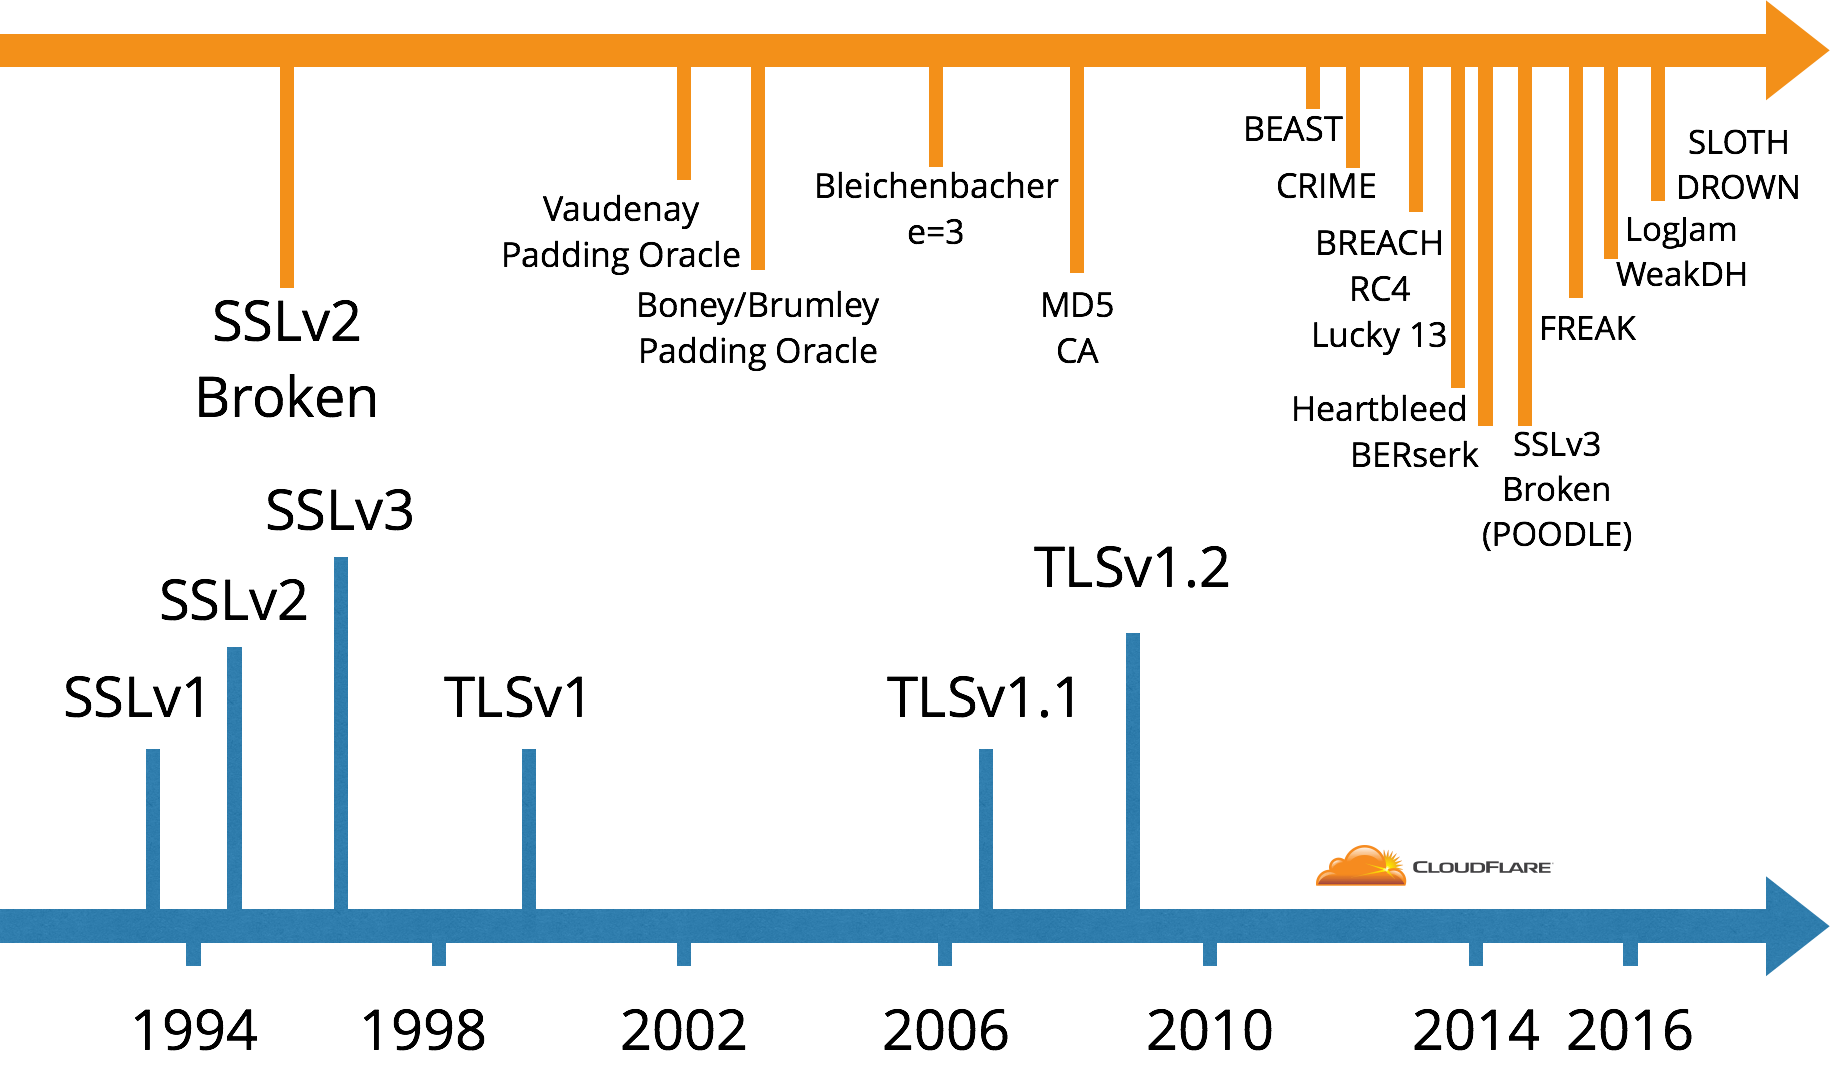
\includegraphics[width=\textwidth]{./history-tls-attacks.png}}
\end{figure}

\section{Attaques liées à l'implémentation}

\subsection{Heartbleed (2014)}

Blablabla \cite{heartbleed}

\section{Attaques liées à la cryptographie}

\subsection{BEAST (2011)}

Blablabla \cite{beast}

\subsection{SWEET32 (2016)}

Blablabla \cite{sweet32}

\section{Attaques sur le protocole}

\subsection{CRIME (2012)}

Blablabla \cite{crime}

\section{Attaques de l'homme du milieu}

\subsection{SSLstrip}

\subsection{SSLsniff}

\subsection{HTTPS interception}
